\chapter{Introduction}\label{ch:intro}
\section{General Introduction}
\subsection{What is a Short Text ?}

Nowadays, customers are used to buy and order products all over the world with only a few clicks on the web. Products are exported and shipped all over the world and these arrive in only a couple of weeks or even days at their destination. This scenario illustrates the enormous increase in global trading over the last decades \cite{EstebanOrtiz-Ospina2018OurGlobalization} and even years \cite{WorldTradeOrganization2019World2019}. To facilitate this massive global trading there is need for a common basis that identifies products. The World Customs Organisation (WCO) has published the ‘language of trade’ by means of the Harmonized System (HS) \cite{WorldOrganization}, which is a nomenclature to classify goods. When the customs authorities are given a product, they classify this to a label that corresponds to that type of product. The label of the product uniquely identifies a product. This is important for governments in terms of the calculation of duties, taxes and fees; determination of permits, license and certificates required and the collection of trade statistics \cite{Ding2015}. In this way, the Harmonized System works as a common basis facilitating trade across more than 200 countries all over the world.\\
\\
Current reports have shown that classifying goods and products according to the Harmonized System is a difficult task. According to the Customs duty of Canada one out of five goods is incorrectly classified \cite{AuditorGeneralofCanada2017}. In addition, it was estimated that the government of Canada missed approximately 21 million dollars due to misclassification in a single year \cite{AuditorGeneralofCanada2017}. A large IT company in the Netherlands (Atos) has the information that authorities have employees that classify goods working 120 FTE per week. Misclassification can occur due to the high number of possible labels, confusing and extensive descriptions of products and the enormous amount of goods to be classified \cite{Kappler2011ReversingPayments}. With this all in mind a way to automatically classify goods can be highly beneficial to the entire process of classification.\\
\\
In the current thesis, research is conducted on an automatic classification of products on a large amount of classes. A large IT company in the Netherlands has provided a dataset containing a wide range of products. This dataset is a collection of descriptions of a product and their corresponding HS-code. Rather than complete English sen- tences these descriptions contain a collection of keywords of the products. Therefore, this research involves experiments of classification on short texts of products. In the field of Natural Language Processing this task is often referred to as text classification in which a document is assigned to classes or categories [7]. Examples are identifying spam emails and sentiment classification of tweets or reviews.\\
\\
Previous research into automatic classification of HS codes rendered promising results in classifying goods [4] [8]. In these recent studies the authors achieve a high accuracy score (> 0.9) in classifying the actual product. However, the task is only carried out on a portion of the labels. In Ding et al. [4] only chapters 22 and 90 were selected because these chapters were most likely to be missclassified in practise. In Li et al. [8] descriptions and images of four classes were selected because classification on all classes was considered extremely difficult. By reducing the amount of classes taken into account, both researches heavily reduced the complexity of the problem. Never- theless, to the best of knowledge, text classification of HS codes with a high number of products has not been done before. Moreover, in this thesis, images of products are not available; as a consequence the authors only focus on classification on the basis of text. Text classification is an active field of study including topic, [9], email [10] and sentiment [11] classification. Therefore, in the current thesis experiments are conducted using a wide range of techniques to classify descriptions of products according to the Harmonized System. The models are grouped in occurrence statistics, hashing and word vectors using a variety of feature extractions and pre-processing techniques of varying complexity, in order to test their advantages and disadvantages for this task.
\\
\\
In Section 2, related work to the problem of text classification is provided. Section 3 describes the system that classifies goods, the so called Harmonized System. In Section 4, the datasets containing a collection of products are introduced. These datasets are real world datasets provided by a customer of Atos and by the Automated Manifest System. In Section 5 the set-up of the experiments in this research is explained. Section 6 includes the implementation of the research and experiments on the hyperparameters. In Section 7 results on the real word datasets are described. A conclusion and outlook are formulated in respectively sections 8 and 9.

\subsection{Short text vs Long text}

\section{Background: The Harmonized System}
The Harmonized System (HS) is a world-wide standard for product classification and sees an almost complete adaption worldwide \cite{}. It is a complex hierarchical system, with multiple levels that divide goods into chapters, headings, and finally subheadings. While the top-most level only contains up to 99 definitions, the system allows for over 5300 precise definitions at level of subheadings. Furthermore, countries have the full liberty to extend upon subheading definition with one or two more levels for their own internal needs \cite{}. Examples of these extensions are the Brazilian NCM and the United States’ HTS. It is important to note that at every level the system is defined by both a code and a textual description, and that at each level the definitions become more detailed.

\subsection{Examples}
In the Harmonized System, a sand-moving diesel-fuel using bulldozer falls under the chapter of nuclear reactors, boilers, machinery and mechanical appliances, or parts thereof. This chapter has the code 84. One level lower is the description of self-propelled bulldozers, angledozers, graders, levellers, scrapers, mechanical shovels, excavators, shovel loaders, tamping machines, and road rollers. The harmonized system code description for this heading is 8429. The system then still goes deeper when defining the subheading group of self-propelled bulldozers and angledozers other than track-laying. This description matches the code 842919. Countries are allowed to extend this system with their own codes, which are added as a suffix to the subheading code (HS-6). This is illustrated in table 1.1.

\begin{center}
    \begin{tabular}{lccccc} \hline \centering
Level & Example Code \\ \hline
Chapter (HS-2) & 84\\
Heading (HS-4) & 8429\\
Subheading (HS-6) & 842919\\
Country-specific extension (HS-8 and beyond) & 84291900\\ \hline
\end{tabular}
\end{center}
{\textit{table 1.1: The hierarchical nature of the Harmonized System demonstrated}} \\

For the sake of consistency, we will refer to these descriptions according to the length of their corresponding HS-code. Thus, the chapter will be referred to as HS-2, the heading as HS-4, and the subheading as HS-6. In the case of country-specific data with a code consisting out of 8 digits, we will refer to these as HS-8. While the classification system includes 21 sections as well as a super-group of chapters, this is outside of the scope of this research as these are not tied to the Harmonized System’s code itself and have limited relevancy for classification.

\subsection{Usage of the Harmonized System}
Upon entering a country, carriers are required to present a customs form for their cargo. An example of such a form is shown in 1.1, with the fields for product descriptions marked. Other countries or custom unions have their own forms, but the general usage is, due to the high degree of adaption of the harmonized system, essentially the same. This form contains information on the shipment, and is often the first item considered when evaluating which shipments should be inspected if it so happens that doubts are raised regarding the truthfulness of the declaration. The form specifically has fields for a text describing the cargo and its corresponding classification, written by traders or agents.
\\
Another example of a HS-code as it is likely to appear in its use for the consumer market can be seen in Figure 1.2. This sticker includes an European Combined Nomenclature (CN) subheading code of eight digits (HS-8) along with a product description. Interestingly, the code consists out of eight digits. This means that we can infer that the product was imported from inside the EU, as imports from outside the EU are given a TARIC code (corresponding to HS-10) instead.\\
\\
Lastly, HS classification codes serve as a way to collect statistics on what is imported and exported to a country. Although this is a significant focus of the Harmonized System, it is outside of the scope of this thesis.\\

\begin{center}
    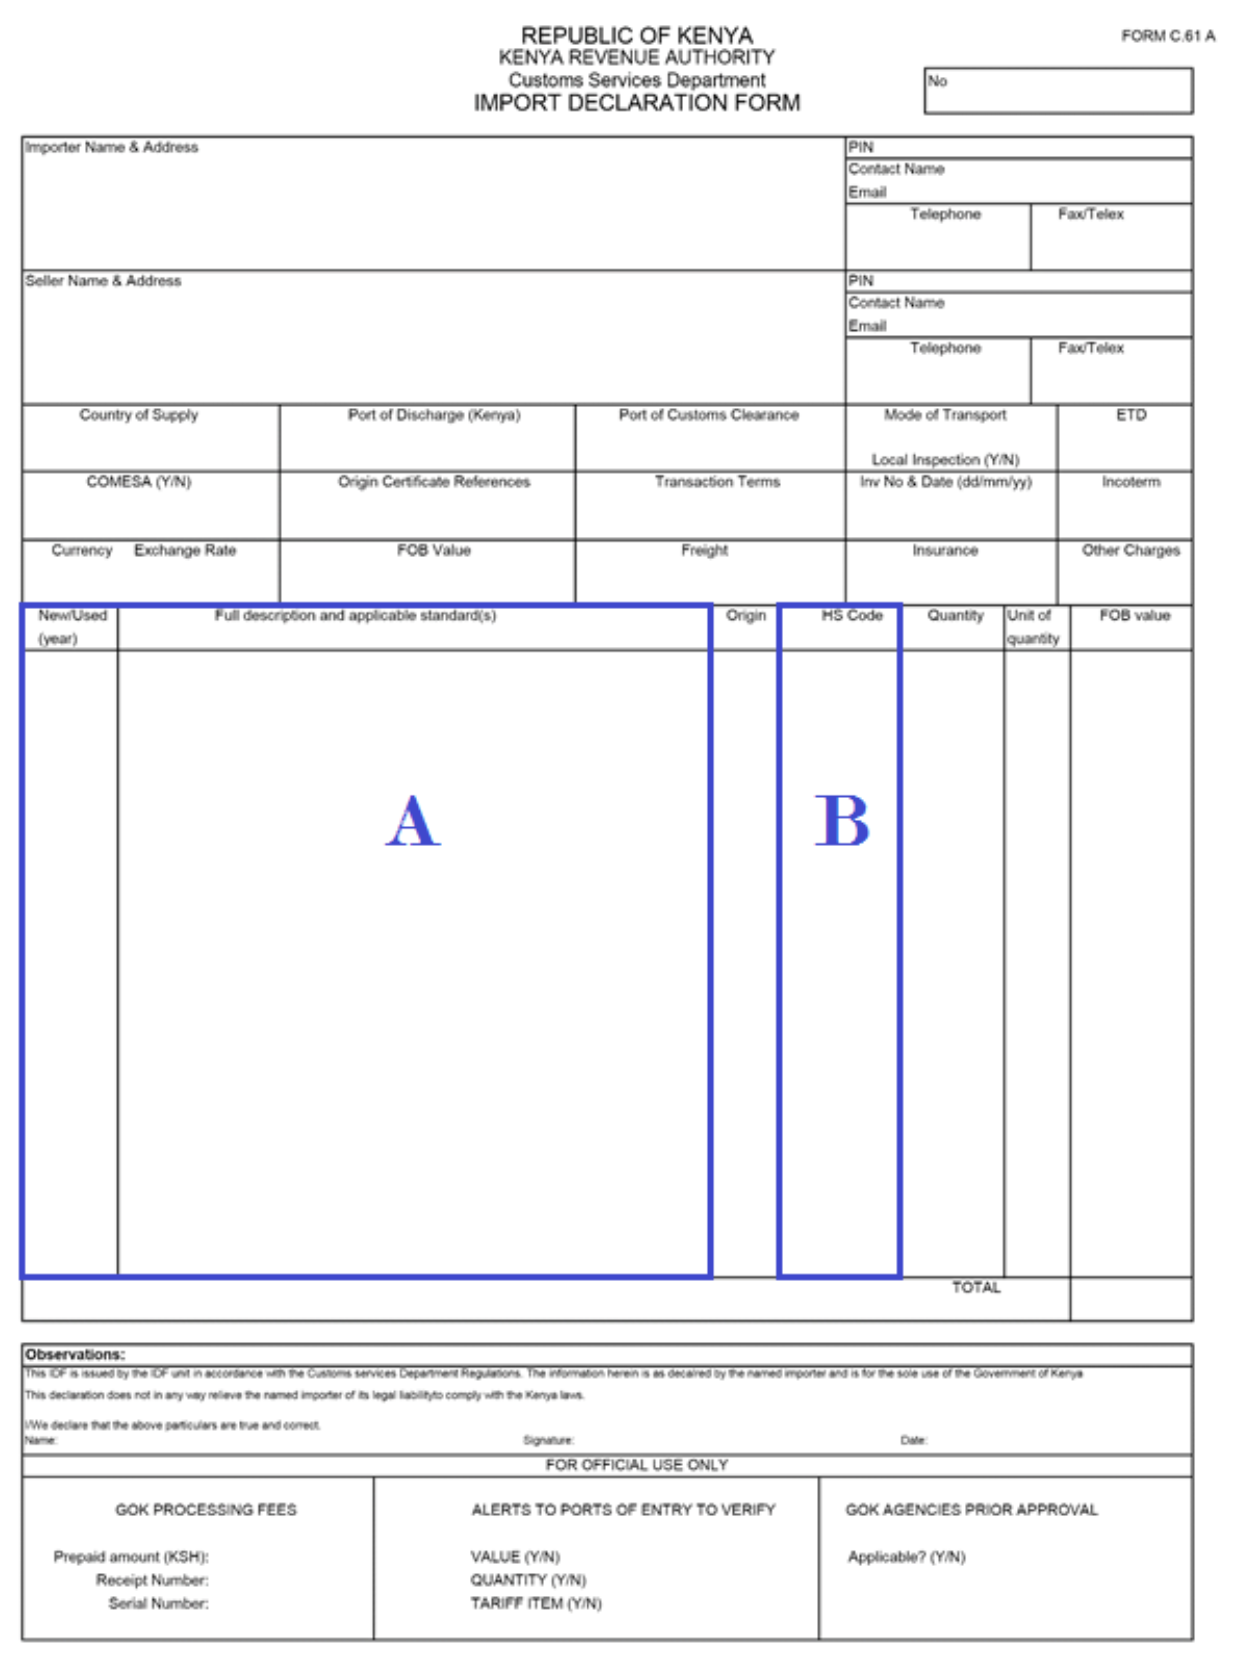
\includegraphics[width=0.8\textwidth]{kenya.png}
\end{center}
{\textit{Figure 1.1: The Kenyan customs form 61a, which is used to declare imports. Outlined are two relevant sections to describe products and assign a HS- code. Forms like these are used world-wide. Section A provides a text field for a product description, and section B provides a field for the HS code. Other fields on the form are not used within this thesis, but one could argue they can easily be utilised to improve performance on classification tasks.}}
\\
\\
\begin{center}
    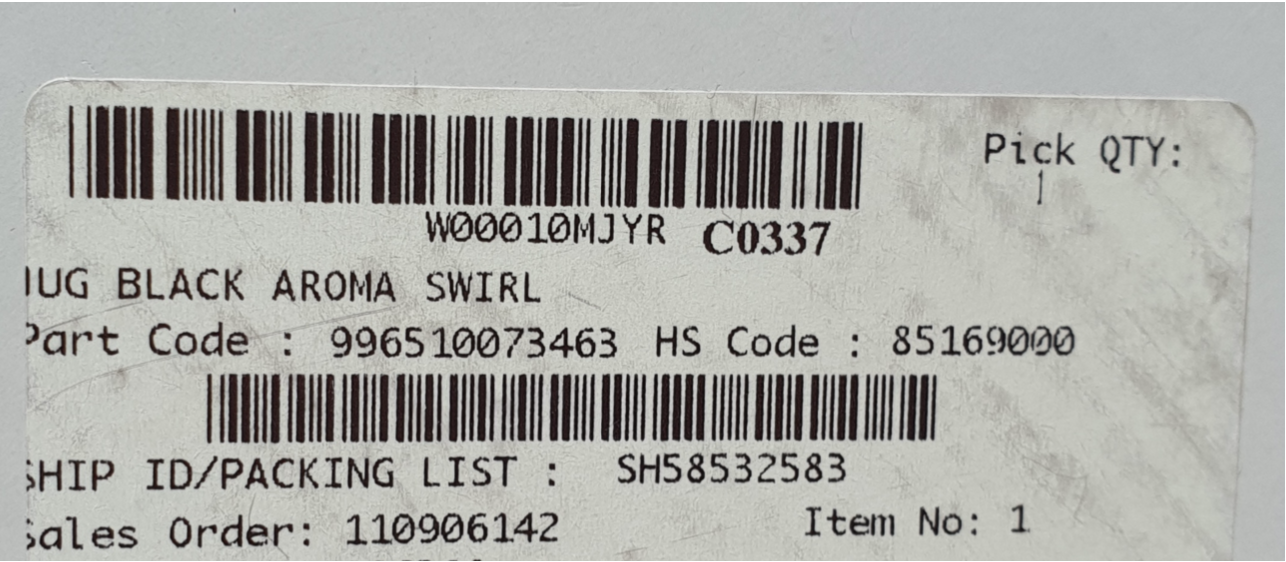
\includegraphics[width=0.8\textwidth]{sticker.png}
\end{center}
{\textit{Figure 1.2: A HS code as it is likely to appear with documents accompanying packages. This sticker contains a textual description (‘JUG BLACK AROMA SWIRL’) and a HS-8 code (85169000) which corresponds to parts of electric instantaneous or storage water heaters and immersion heaters; electric space-heating apparatus and soil-heating apparatus; electrothermic hairdressing apparatus (for example, hairdryers, hair curlers, curling tong heaters) and hand dryers; electric smoothing irons; other electrothermic appliances of a kind used for domestic purposes; electric heating resistors, other than those of heading 8545. The item imported was a coffee pot.}}
